\chapter{The LHCb experiment}
\label{cap:LHCb}

\section{The Large Hadron Collider}
\label{sec:2:lhc}

\begin{figure}[t]
	\centering
	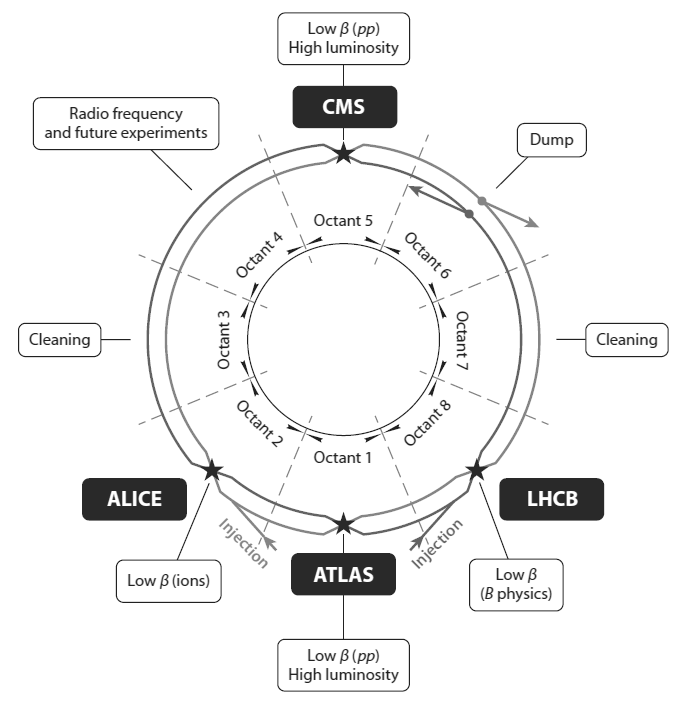
\includegraphics[width=.6\textwidth]{graphics/02-lhcb/lhc_diagram.png}
	\caption[LHC schematic layout.]{Layout of the Large Hadron Collider with its four main experiments \cite{doi:10.1146/annurev-nucl-102010-130438}.}
	\label{fig:2:lhc_diagram}
\end{figure}

At the moment of writing, the Large Hadron Collider (LHC for short) is the largest and most powerful particle collider in the world.
When the LHC was first approved by the European Organization for Nuclear Research (CERN) in 1994, it was originally going to be built with an initial center-of-mass collision energy $\sqrt{s} = \SI{10}{\tev}$, with the plan to upgrade it to \SI{14}{\tev} at a later stage;
however, after negotiations with nonmember states, in 1996 the CERN council approved the construction at \SI{14}{\tev} energy in one stage \cite{doi:10.1146/annurev-nucl-102010-130438}.
%First collisions were obtained in 2010 at center-of-mass energy of \SI{7}{\tev}, with the current world record of \SI{13}{\tev} being achieved in 2015 after the first Long Shutdown.

LHC is located at the CERN laboratory near Geneva, Switzerland, housed in the underground tunnel previously occupied by the LEP experiment.
Its structure, sketched in Figure \ref{fig:2:lhc_diagram}, consists of two counterrotating rings hosting beams for particle-particle collisions (mainly protons, but LHC is also used for ion collisions).

Four main experiments are stationed at the LHC ring intersection points:
ATLAS and CMS are high-luminosity experiments focused on general purpose proton-proton collisions; ALICE is optimized for lead-on-lead collisions with lower center-of-mass energy and luminosity compared to the former two; finally, LHCb is dedicated on the study of $b$ hadrons and will be the focus of the rest of this chapter.
Beyond the above four, a number of small-scale, more specialized experiments also work with LHC, such as TOTEM, MilliQan and MoEDAL.

%Broadly speaking,
The LHC schedule alternates data collection phases (\textit{Runs}) with maintenance work phases (\textit{Long Shutdowns}, LS for short);
while the shutdowns are designed for consolidation and improvement of the collider itself, mainstay experiments usually take advantage of the hiatus to upgrade their detectors in both hardware and software.
Run 1 began in 2010 and continued until early 2013, during which period the LHC provided a center-of-mass energy of $\sqrt{s} = 7$--$8$ \si{\tev}.
After the 2-year-long interruption for LS1, operations resumed in 2015 for Run 2 with an upgraded $\sqrt{s} = \SI{13}{\tev}$.
The collider was once again shut down at the end of 2018 (LS2) and work began towards the High Luminosity (HiLumi) upgrade of the LHC.
After suffering delays due to the COVID-19 pandemic, Run 3 is currently scheduled to start in the second quarter of 2022 with $\sqrt{s} = \SI{14}{\tev}$, finally reaching its maximum collision energy by design.


\section{The LHCb experiment and detector}
\label{sec:2:lhcb_detector}

\begin{figure}[t]
	\centering
	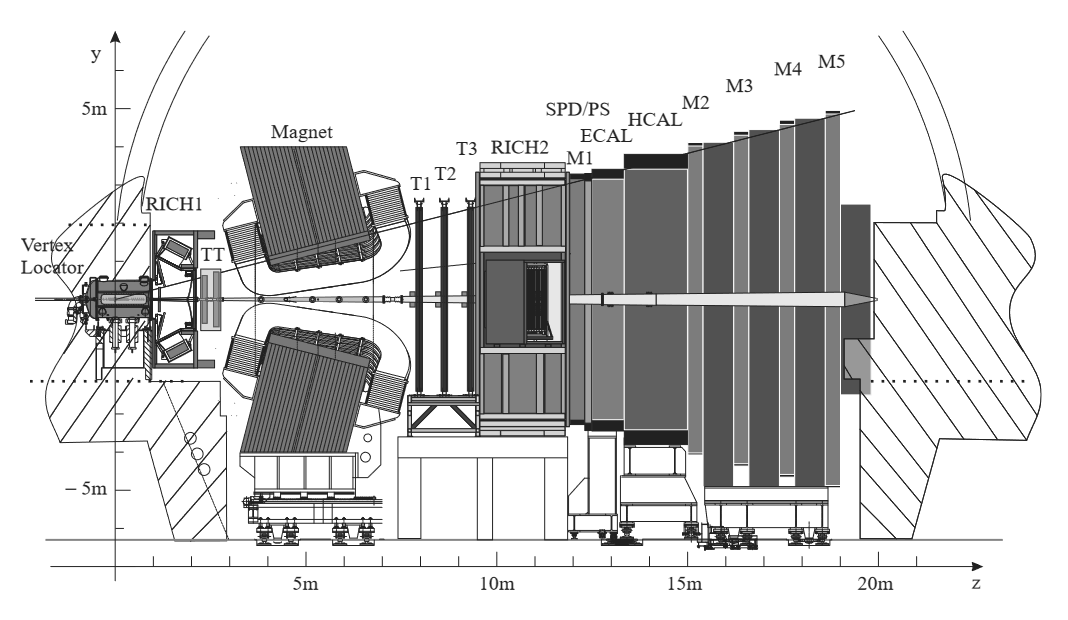
\includegraphics[width=\textwidth]{graphics/02-lhcb/lhcb_diagram.png}
	\caption[LHCb detector side view (Runs 1 and 2).]{Side view of the LHCb detector used for LHC Runs 1 and 2 \cite{Antunes-Nobrega:630827}.}
	\label{fig:2:lhcb_diagram}
\end{figure}

LHCb (the \textit{b} stands for \textit{beauty}\footnote{Before settling on the names \textit{top} and \textit{bottom} for the third generation of quarks, the names \textit{truth} and \textit{beauty} were among those proposed. While they never gained enough momentum in the scientific community, echoes of the failed nomenclature are still present in heavy quark vocabulary, for instance in the alternative name \textit{truth} for the \textit{topness} flavour number mentioned in Section \ref{sec:flavour-physics}, as well as in the official name for the LHCb experiment.}) is a single-arm detector designed to study heavy-flavour physics at the LHC, with the main objective of providing precision measurements of CP violation and rare decays of $b$ and $c$ hadrons \cite{Alves:1129809}.

Unlike the other three main experiments at LHC, LHCb has a forward-optimized geometry shown in Figure \ref{fig:2:lhcb_diagram}, with an angular acceptance of 10--300 \si{\mrad} in the bending plane and 10--250 \si{\mrad} in the non-bending plane.
%\footnote{For the sake of brevity, I'll refer to it as the 300/250 \si{\mrad} acceptance or the.}
Such a layout, more reminiscent of fixed target experiments than beam colliders, is motivated by the fact that $b\bar{b}$ pairs produced at high energies are usually collimated in the same forward/backward cone.
A more in-depth look at the tracking and particle identification systems will be taken in Sections \ref{sec:2:tracking} and \ref{sec:2:pid} respectively.
\label{info:LHCb_system}
The standard LHCb coordinate system, used as reference for the rest of this thesis, is a right-handed system centered on the beam interaction point, with the $z$ axis along the the beam pipe and $y$ axis directed vertically upwards.

By all accounts, LHCb has been an incredibly successful experiment, reaching its 600th publication by the end of 2021 and leading to state-of-the-art results both within and outside of its intended research framework.
Among the main results achieved by the LHCb Collaboration in the field of CP symmetry violation are world-class precision measurements of heavy quark mixing \cite{B0MeasurementPrecise2016} \cite{B0MeasurementPrecise2013}, the first observation of CP violation in the charm sector \cite{PhysRevLett.122.211803} and competitive measurements of the CKM unitarity triangle parameters \cite{LHCb-CONF-2020-003}.
LHCb has also been active in the study of rare $b$-hadron decays \cite{PhysRevLett.118.191801}, as well as in conventional and exotic hadron spectroscopy \cite{DMesonSpectroscopy}, particularly concerning evidences of new pentaquark states \cite{LHCbPentaquark}.
Finally, LHCb has the distinction of being the only current LHC experiment with the ability to use a fixed-target setup by exploiting the SMOG internal gas target \cite{maurice2017fixedtarget}, originally developed for precise luminosity measurements;
ever since 2015, the adoption of noble gas targets has allowed the Collaboration to obtain $b$-physics results involving nuclear collisions \cite{PhysRevLett.122.132002}.


\subsection{Tracking}
\label{sec:2:tracking}
In order to measure the momenta of charged particles through their bending curve, LHCb employs a dipole magnet \cite{Amato:424338} consisting of two trapezoidal coils bent at $45^\circ$ on the two transverse sides, seen in Figure \ref{fig:2:lhcb_diagram} around $z\approx \SI{5}{\meter}$ (the magnet is placed so that the line connecting the centers of the pole faces crosses $z=\SI{5.3}{\meter}$).

\begin{figure}[t]
	\centering
	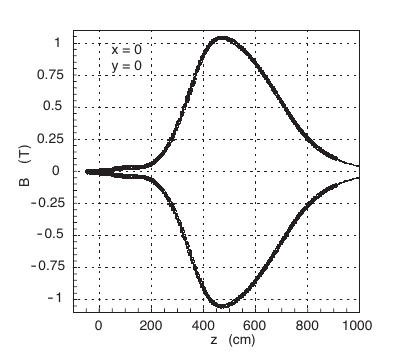
\includegraphics[width=.6\textwidth]{graphics/02-lhcb/b_field_map_z.png}
	\caption[LHCb magnetic field along the $z$ axis.]{LHCb magnetic field along the $z$ axis \cite{Amato:424338}.}
	\label{fig:2:b_field_map_z}
\end{figure}

This magnet provides an integrated field of $\int B dl \approx \pm \SI{4}{\tesla\meter}$ for \SI{10}{\meter} tracks\footnote{The $\pm$ sign is due to the fact that the magnet operates alternatively in up and down polarities, inverting the sign of the magnetic field.}.
Most of this field is contained in the $z\in[2.5,7.95]$ \si{\meter} region, with 
a small fraction ($\int B dl \approx \SI{0.12}{\tesla\meter}$) upstream of $z=\SI{2.5}{\meter}$. The field map along $z$, measured with a precision of $4 \times {10}^{-4}$, is shown in Figure \ref{fig:2:b_field_map_z} for $x=y=0$.
Dishomogeneities in the $xy$ plane for fixed $z$ are estimated at $\lesssim 6\%$ within the LHCb detector acceptance.

\subsubsection{VELO}
As the name suggests, the VErtex LOcator (VELO) system \cite{Barbosa-Marinho:504321} is designed to provide precision measurements of charged tracks near the beam interaction point, in order to correctly reconstruct detached secondary vertices typical of $b$- and $c$-hadron decays.

\begin{figure}[t]
	\centering
	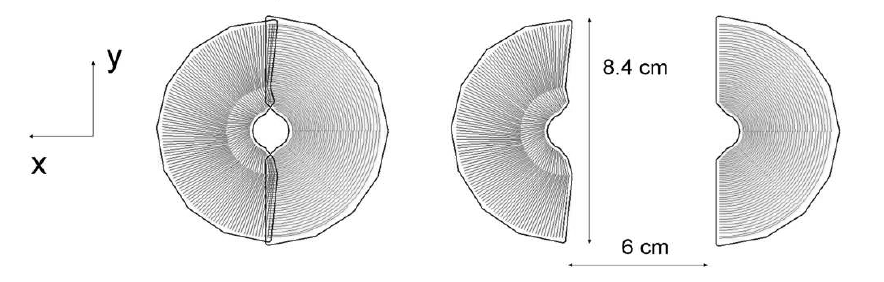
\includegraphics[width=\textwidth]{graphics/02-lhcb/VELO_xy.png}
	\caption[Front view diagram of the VELO detector.]{Front view diagram of the VELO detector in fully closed (\textit{left}) and fully open (\textit{right}) configurations \cite{Barbosa-Marinho:504321}.}
	\label{fig:2:VELO_xy}
\end{figure}

The VELO detector comprises 42 silicon modules along the beam direction, each consisting of a pair of half discs measuring the radial and azimuthal track coordinates respectively. These modules cover the $1.6 < \eta < 4.9$ positive pseudorapidity range, as well as some negative pseudorapidity portion to improve primary vertex reconstruction, and are able to detect particles emerging from primary vertices with $|z| < \SI{10.6}{\centi\meter}$.
Due to high risk of radiation damage during beam injection from the Super Proton Synchrotron (SPS) into LHC, these modules can be retracted by \SI{3}{\centi\meter} in so-called \textit{fully open} configuration, whereas during collision phase the VELO operates in \textit{fully closed} configuration (see Figure \ref{fig:2:VELO_xy}).

\begin{figure}[t]
	\centering
	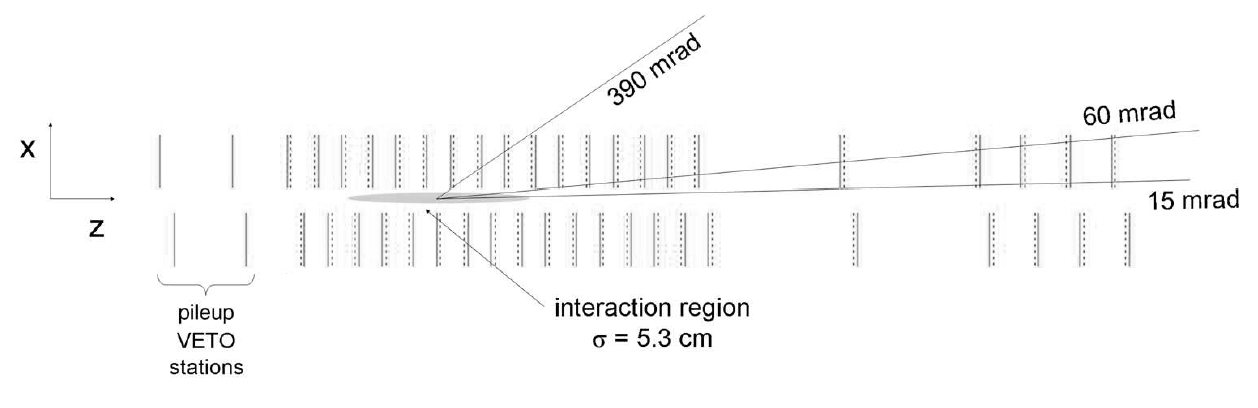
\includegraphics[width=\textwidth]{graphics/02-lhcb/VELO_xz.png}
	\caption{Cross-section diagram of the fully closed VELO detector in the $xz$ plane at $y=0$ (top view). Radial sensors are depicted as \textit{solid} segments, azimuthal sensors as \textit{dashed} segments \cite{Barbosa-Marinho:504321}.}
	\label{fig:2:VELO_xz}
\end{figure}

Figure \ref{fig:2:VELO_xz} shows the $xz$ plane cross-section of the VELO modules; the two halves of the detector are $z$-shifted by \SI{1.5}{\centi\meter} to ensure full azimuthal acceptance, resulting in the partial overlap seen in fully closed configuration.
Four radial-only \textit{pile-up sensors}, part of the Level-0 hardware trigger system (see Section \ref{sec:2:data_flow}), are placed upstream to help veto multiple-interaction events.



\subsubsection{Tracker Turicensis}
The Tracker Turicensis (TT) \cite{Gassner:728548}, formerly known as Trigger Tracker, is a $\SI{150}{\centi\meter} \times \SI{130}{\centi\meter}$ tracking station located just upstream of the dipole magnet.
Its placement serves the main purpose of tracking low-momentum particles ($|\vec{p}| \lesssim \SI{1.5}{\gev\per c}$) that would otherwise be bent out of the detector by the magnet without reaching the T stations.

The TT consists of four readout layers of silicon microstrip sensors arranged in a $x$-$u$-$v$-$x$ configuration (vertical in the first and last layers, rotated by a stereo angle of $\mp 5^\circ$ in the second and third layer respectively) for a total active area of $\approx \SI{8.4}{\meter\squared}$.
A \SI{200}{\micro\meter} strip pitch ensures a single-hit resolution $\lesssim \SI{50}{\micro\meter}$.

\begin{figure}[t]
	\centering
	\includegraphics[width=.6\textwidth]{graphics/02-lhcb/TT_layout.png}
	\caption[Front view of the third TT layer.]{Front view of the third TT layer (different readout sectors are labeled with different shadings) \cite{Alves:1129809}.}
	\label{fig:2:TT}
\end{figure}

The third TT layer is depicted in front view in Figure \ref{fig:2:TT}.
The basic unit of a layer is the \textit{half module}, covering half the LHCb height acceptance.
Each half module consists of a row of seven sensors bonded together to form either three or two \textit{readout sectors}.
Modules near the beam pipe are of the former category, with four sensors bonded in the L sector, two in the intermediate M sector and a single sensor for the K sector closest to the beam ($4$--$2$--$1$ modules);
other modules forgo the K sector and bond the spare sensor in the M sector ($4$--$3$ modules).
Front-end readout hybrids, one for each sector, are placed at the L-end of the half modules, outside of the detector acceptance, connected directly to the L sector and indirectly to the M and K sectors via Kapton flex cables.

\subsubsection{T stations}
\begin{figure}[t]
	\centering
	\begin{subfigure}{.45\textwidth}
		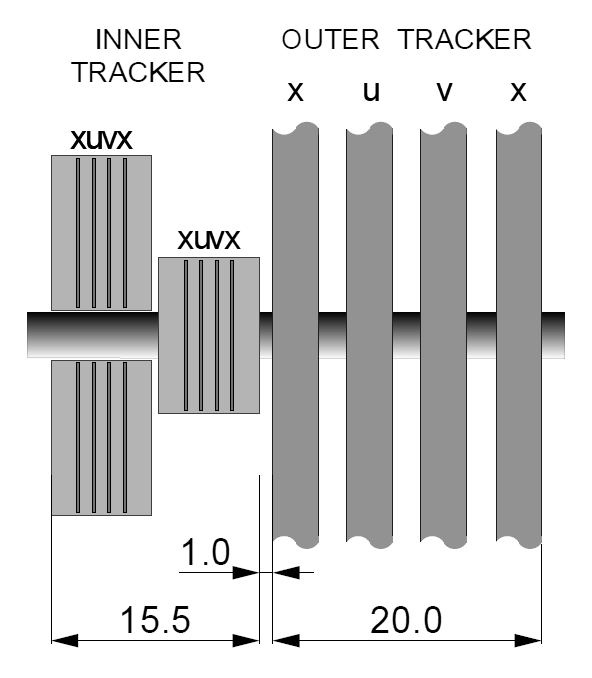
\includegraphics[width=\textwidth]{graphics/02-lhcb/t_station_top_view.png}
		\caption{}
		\label{fig:2:t_station_top}
	\end{subfigure}
	\begin{subfigure}{.45\textwidth}
		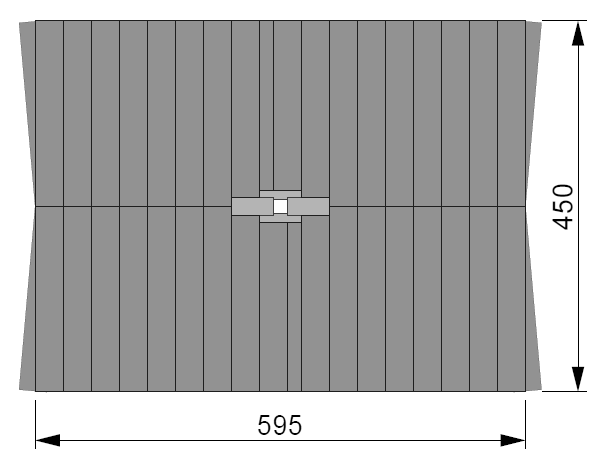
\includegraphics[width=\textwidth]{graphics/02-lhcb/t_station_front_view.png}
		\caption{}
		\label{fig:2:t_station_front}
	\end{subfigure}
	\caption[Top and front views of a T tracking station.]{Top (\textit{left}) and front (\textit{right}) views of a T tracking station \cite{Barbosa-Marinho:582793}. IT and OT are labeled with lighter and darker shades of grey respectively. Dimensions are given in \si{\centi\meter}; for the top view, lateral dimensions are not to scale.}
	\label{fig:2:t_station}
\end{figure}

The three T stations, labeled as T1--T3, are the last line of defense for LHCb tracking purposes, covering the $z \approx 7.7$--$9.4\,\si{\meter}$ region downstream of the dipole magnet \cite{Barbosa-Marinho:582793}.
Each T station is composed of an Inner Tracker for the region near the beam pipe and an Outer Tracker for the farther regions, as sketched in Figure \ref{fig:2:t_station}.

\begin{figure}[t]
	\centering
	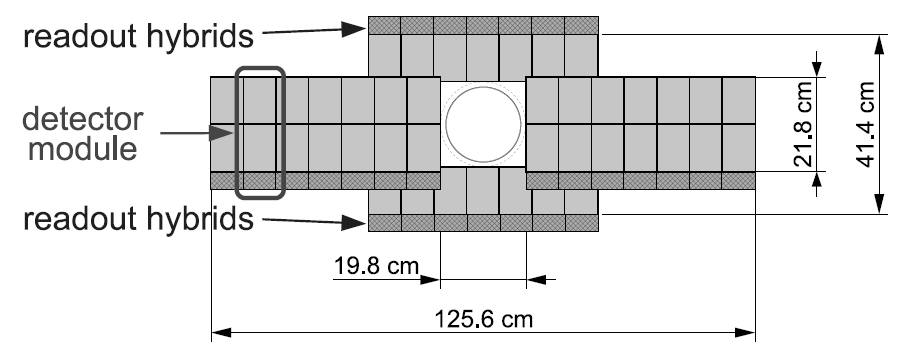
\includegraphics[width=.6\textwidth]{graphics/02-lhcb/it_layout.png}
	\caption[Front view of an Inner Tracker $x$ layer.]{Front view of an $x$ detector layer in the T2 Inner Tracker \cite{Alves:1129809}.}
	\label{fig:2:IT}
\end{figure}

The Inner Tracker (IT) \cite{Barbosa-Marinho:582793} shares many similarities with the TT design, being developed in conjuction with it under the common Silicon Tracker (ST) project.
Sporting the same four layers of silicon microstrips in $x$-$u$-$v$-$x$ configuration, it covers a comparatively smaller $\SI{120}{\centi\meter} \times \SI{40}{\centi\meter}$ cross-shaped surface (see Figure \ref{fig:2:IT}) for a total active area of $\approx \SI{4}{\meter\squared}$, less than half the TT.
As a consequence, individual modules only include one or two sensors  connected to the readout hybrids via a pitch adapter.

The much larger Outer Tracker (OT) \cite{Barbosa-Marinho:519146} is a drift detector consisting of an array of Ar/CO$_2$ straw-tube modules.
Each module contains two layers of straw tubes with \SI{4.9}{\milli\meter} inner diameter, ensuring a \SI{50}{\nano\second} drift time and \SI{200}{\micro\meter} spatial resolution.
Within a single T station, said modules are arranged in four layers in $x$-$u$-$v$-$x$ configuration (see Figure \ref{fig:2:t_station_top}) with $\pm 5^\circ$ vertical tilt for $u$ and $v$ layers respectively.
The OT covers the entire 300/250 \si{\milli\rad} LHCb detector acceptance.

\subsubsection{Track classification and the problems with T tracks}
Overall, the LHCb tracking system has very high efficiency, besting $96\%$ in the momentum range $|\vec{p}|=5$--$200$ \si{\gev\per c} for tracks crossing all three detector stations (VELO, TT and T1--T3) \cite{HistoryLHCb}. 
However, not all particles enjoy this luxury:
low momentum particles ($|\vec{p}| \lesssim \SI{1.5}{\gev\per c}$) are unable to reach the T stations due to the sharp magnet bending curve, while daughters of longer-lived particles with $c\tau \gtrsim \SI{30}{\centi\meter}$ will miss the VELO and possibly even the TT detector.

\begin{figure}[t]
	\centering
	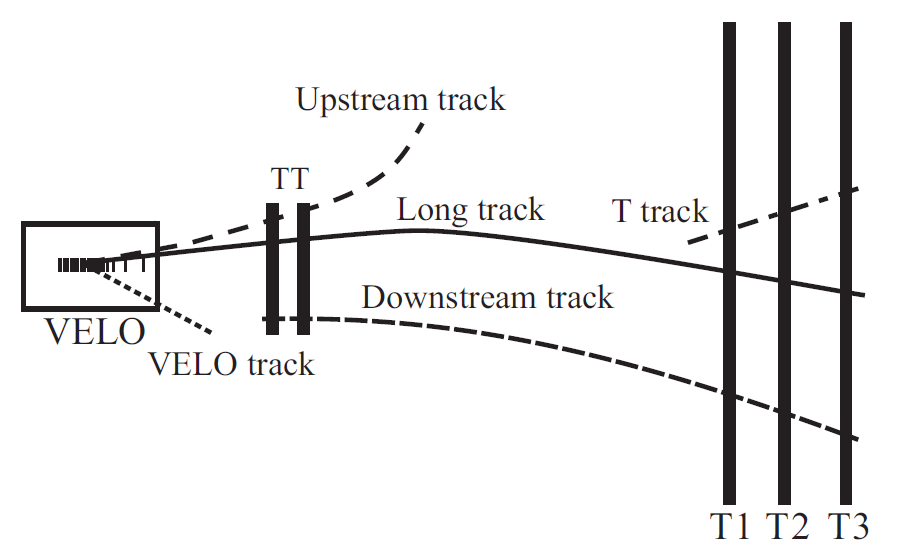
\includegraphics[width=.8\textwidth]{graphics/02-lhcb/Track_Definitions.png}
	\caption[Side view diagram of LHCb tracking system and track categories.]{Side view diagram of the LHCb tracking systems for LHC Runs 1 and 2 with sketched examples of the main track classification categories.}
	\label{fig:2:track_classification}
\end{figure}

Thus, in spite of the great efficiency, it's useful to define track categories in the LHCb working environment depending on what hits were recorded in which detectors:
\begin{itemize}
	\item \textit{Long} tracks are reconstructed from hits in the VELO and T stations, with TT hits being optional. They are the most commonly used tracks for physics analysis in LHCb, exploiting the full performance of the detector tracking system; the long distance between VELO and T detectors means that only stable or quasi-stable charged particles can aim for this classification.
	\item \textit{Upstream} tracks are reconstructed from hits in the VELO and TT detectors. As previously discussed, low-momentum particles usually fall in this category due to inability to reach the T stations.
	\item \textit{VELO} tracks are reconstructed from hits in the VELO detector alone. These are often large-angle or backward tracks, valuable to correctly identify the primary vertex of the event.
	\item \textit{Downstream} tracks are reconstructed from hits in the TT and T1--T3 detectors. This is the most common category to study long-lived particles (LLP) decaying after the VELO, such as \lz baryons and $K_S^0$ mesons.
	\item \textit{T} tracks are only reconstructed from hits in the three T stations. Since missing both VELO and TT is a rare occurrence, these tracks largely come from LLPs with $c\tau \gtrsim \SI{5}{\meter}$ decaying after the dipole magnet.
\end{itemize}
Sketches of tracks satisfying the above requirements are depicted in Figure \ref{fig:2:track_classification}.

Among the four, T tracks have seen the least use over LHC Runs 1 and 2.
The main reason is related to their key property of only having measured constraints after the magnet:
in order to reconstruct their origin vertex, T tracks have to be extrapolated through several meters of intense magnetic field, an operation that has ripercussions in terms of both accuracy and timing.
On top of that, the further a charged particle is produced after the dipole magnet, the less the residual magnetic field will be able to imprint a significant bending radius, negatively affecting the momentum resolution at T station level.

Over the ten years of detector operation there has been little physics incentive to fix or mitigate these issues, as most LLPs relevant to LHCb can already be studied using Downstream tracks.
The \lz EDM/MDM measurement proposal outlined in Section \ref{sec:lambda} is one of the atypical cases where T tracks are downright essential, since the technique hinges on the measurement of the spin precession of the baryon traversing the magnetic field before decaying in the $p\pi^-$ pair.
Over the course of the following chapters, I'll delve into more detail on the approaches adopted to overcome the problems associated with T tracks in view of competitive measurements of the \lz electromagnetic dipole moments.


\subsection{Particle identification}
\label{sec:2:pid}
While tracking outgoing particles is obviously of paramount importance for physics analysis, knowledge of \textit{what} particles are being tracked is also crucial.
The ability to distinguish protons, pions and kaons is of particular interest at LHCb due to its research objectives in CP violation and $b$ physics, requiring precise flavour tagging and physical background rejection.
For the above reasons, a complex ecosystem of detectors dedicated to particle identification (PID) is in place.

\subsubsection{RICH}
Roughly $90\%$ of pions, protons and kaons from $B$ meson decays have momentum in the 2--150 \si{\gev\per c} range \cite{HistoryLHCb}.
Since their momentum distributions depend on the polar angle of production, LHCb employs two Ring Imaging CHerenkov (RICH) detectors \cite{Amato:494263} to cover the full momentum range for these particles.

\begin{figure}[t]
	\centering
	\begin{subfigure}{.45\textwidth}
		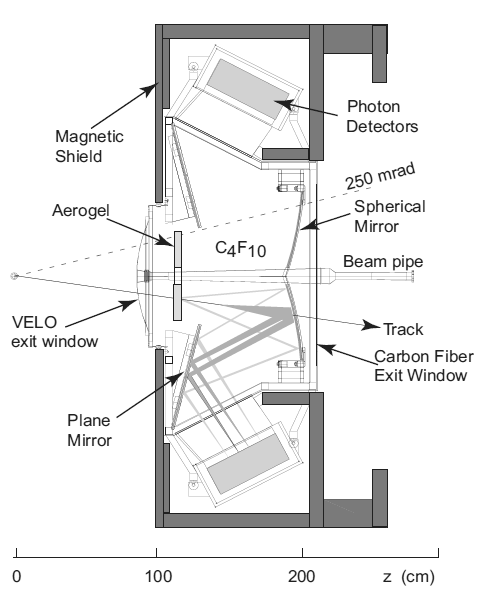
\includegraphics[height=.3\textheight]{graphics/02-lhcb/rich1_top.png}
		\caption{}
		\label{fig:2:rich_1_top}
	\end{subfigure}
	\begin{subfigure}{.45\textwidth}
		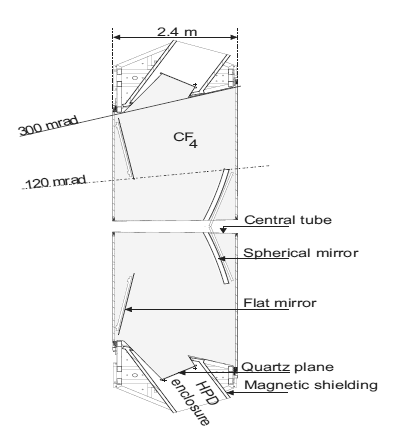
\includegraphics[height=.3\textheight]{graphics/02-lhcb/rich2_top.png}
		\caption{}
		\label{fig:2:rich_2_top}
	\end{subfigure}
	\caption[Top view of the two RICH detectors.]{Top view of the RICH 1 (\textit{left}) and RICH 2 (\textit{right}) detectors \cite{Alves:1129809}.}
	\label{fig:2:rich_top}
\end{figure}

The RICH 1 detector, sketched in Figure \ref{fig:2:rich_1_top}, is located upstream of the dipole magnet, wedged between the VELO and TT tracking detectors.
The detector exploits the different spectra of Cherenkov angles as a function of momentum for different kinds of particles.
During Run 1, RICH 1 used two radiator materials: an aerogel layer ($n=1.03$) and a C$_4$F$_{10}$ gas layer ($n=1.0014$).
This allowed RICH 1 to perform $\pi/K$ identification in the $1$--$60$ \si{\gev\per c} range.
Due to occupancy problems, the silica aerogel radiator providing identification in the low momentum range $|\vec{p}| \lesssim \SI{10}{\gev\per c}$ was removed for Run 2;
since the kaon Cherenkov threshold in C$_4$F$_{10}$ is $\approx \SI{9.7}{\gev\per c}$, they can still be identified by operating RICH in so-called \textit{kaon veto mode}, whereby kaons are marked by the lack of Cherenkov light \cite{HistoryLHCb} \cite{RichPerformance}.
RICH 1 covers from $\SI{25}{\mrad}$ (lower limit imposed by the beryllium beam pipe section) up to the full LHCb acceptance.

Acting as complement to its partner, RICH 2 (Figure \ref{fig:2:rich_2_top}) operates downstream of the T tracking stations and is optimized for a high momentum range, providing PID from $\approx \SI{15}{\gev\per c}$ up to and beyond $\SI{100}{\gev\per c}$.
Its lower limit of acceptance is $\approx \SI{15}{\mrad}$, dictated by the required clearance of \SI{45}{\milli\meter} around the beam pipe.

\subsubsection{Calorimeter}
\begin{figure}[t]
	\centering
	\begin{subfigure}{.45\textwidth}
		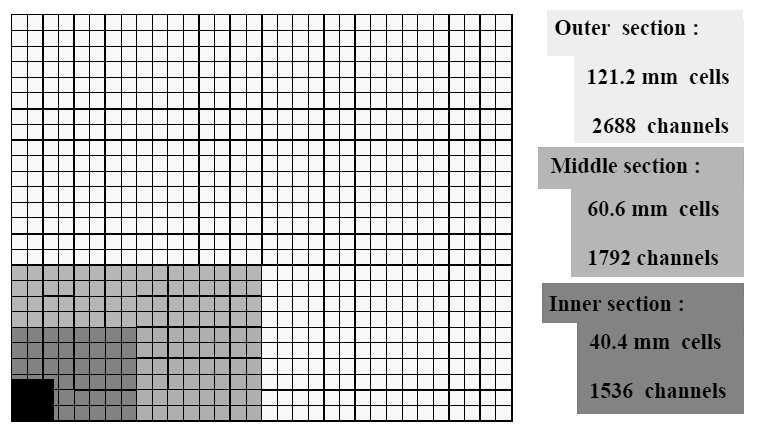
\includegraphics[width=\textwidth]{graphics/02-lhcb/ecal_segm.png}
		\caption{}
		\label{fig:2:ecal_segm}
	\end{subfigure}
	\begin{subfigure}{.45\textwidth}
		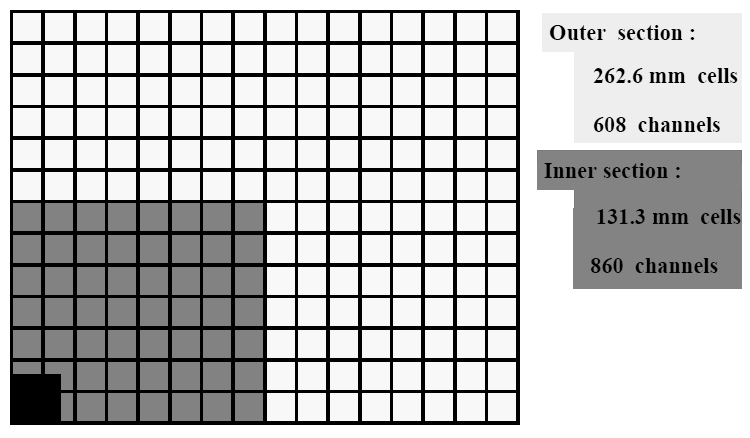
\includegraphics[width=\textwidth]{graphics/02-lhcb/hcal_segm.png}
		\caption{}
		\label{fig:2:hcal_segm}
	\end{subfigure}
	\caption[Front view of the lateral segmentation of SPD/PS, ECAL and HCAL calorimeters.]{Front view of the lateral segmentation of SPD/PS and ECAL (\textit{left}) and HCAL (\textit{right}) calorimeters \cite{Alves:1129809}. Only a quarter of the detector is depicted. Dimensions are given for the ECAL in the left figure.}
	\label{fig:2:ecal_hcal_segm}
\end{figure}

The LHCb calorimeter system \cite{Amato:494264} serves the dual purpose of identifying hadrons, electrons and photons and measuring their energies.
Its design follows the standard high energy physics approach of an electromagnetic calorimeter (ECAL) for the detection of electrons and photons, followed by a hadronic calorimeter (HCAL) for the detection of charged and neutral hadrons.

Placed at \SI{12.5}{\meter} from the beam interaction point, the ECAL employs a shashlik layout\footnote{The nomenclature references the \textit{shashlik}, or \textit{šašlyk}, a traditional meat dish consisting of skewers threaded with alternating pieces of meat, fat and vegetables. The dish is popular throughout the Caucasus and Central Asia regions, including the former Soviet Union, where the shashlik calorimeter technology was first developed.}, alternating layers of absorber (\SI{2}{\milli\meter} thick lead) and sampler (\SI{4}{\milli\meter} thick polystyrene scintillator tiles) perpendicular to the beam axis.
Due to the steep dependence of hit density from the distance from the beam pipe, the calorimeter adopts a variable cell size and is segmented in three distinct sections outlined in Figure \ref{fig:2:ecal_segm}.
The ECAL is approximately $25X_0$ long, with $X_0$ being the radiation length; this allows for the full containment of electromagnetic showers from high energy photons, which is of paramount importance for energy resolution.

Electron detection is particularly tricky due to the significant pion background, both of the charged and neutral variety.
To combat this, two ancillary detectors are located upstream of the ECAL proper: the scintillator pad detector (SPD) selects charged particles to veto $\pi^0$, while the preshower detector (PS) rejects $\pi^\pm$.
Collectively, the SPD/PS detectors consist of two scintillator pads enclosing a \SI{15}{\milli\meter} thick lead plate with a $\SI{7.6}{\meter} \times \SI{6.7}{\meter}$ sensitive area.
Transverse segmentation is designed to projectively match the ECAL segmentation down to the individual cell size.

The HCAL is a sampling calorimeter as well, employing iron as absorber and scintillating tiles as active material.
In contrast to the ECAL and SPD/PS detectors, however, the scintillating tiles run parallel to the beam axis, interspersed with \SI{1}{\centi\meter} thick layers of iron;
meanwhile, the longitudinal structure alternates scintillating tiles with iron spacers, both of length $\lambda_I \approx \SI{20}{\centi\meter}$, $\lambda_I$ being the hadron interactiorn length in steel.
The transvese segmentation of the detector, sketched in Figure \ref{fig:2:hcal_segm}, envisages one less section and a comparatively larger cell size than ECAL, owing to the differing sizes of electromagnetic and hadronic showers.
Since competitive hadron energy resolution does not require full containment of the shower, the HCAL only extends for $\approx 5.6$ interaction lengths.

In all four subdetectors, scintillating light is conveyed through wavelength-shifting fibres to photomultiplier tubes for conversion and magnification; due to the lower light yield of HCAL modules, their phototubes operate at a higher gain.

\subsubsection{Muon system}

The final components of the PID system are the five muon stations M1--M5 \cite{Barbosa-Marinho:504326}, providing trigger and limited tracking for muons in LHCb.
Stations M2--M5 are placed downstream of the calorimeter system, separated from each other by \SI{80}{\centi\meter} of iron;
these absorber layers select muons on the basis of penetration, with a \SI{6}{\gev\per c} momentum threshold required to cross the fifth station.
The lone M1 station precedes the calorimeter system with the goal of improving transverse momentum measurement.
The muon system provides acceptance in the $20$--$306$ \si{\mrad} region in the bending plane and $16$--$258$ \si{\mrad} region in the non-bending plane, in line with the global LHCb acceptance.

\begin{figure}[t]
	\centering
	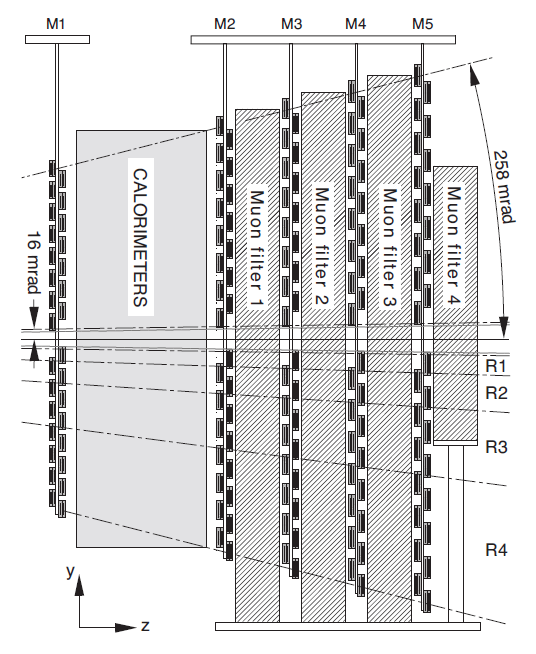
\includegraphics[width=.5\textwidth]{graphics/02-lhcb/muon_side_view.png}
	\caption[Side view diagram of the muon system.]{Side view diagram of the muon system \cite{Alves:1129809}.}
	\label{fig:2:muon_side_view}
\end{figure}


A side view diagram of the muon system is depicted in Figure \ref{fig:2:muon_side_view}: each station is divided in four R1--R4 regions with increasing distance from the beam pipe.
While transverse spatial resolution progressively worsens in outer regions, the growing influence of large angle multiple scattering means it would be limited anyway.

The most sensitive area is the R1 region of the M1 station, since the large particle flux imposes strict limits on radiation hardness to prevent ageing effects during the LHC projected lifetime.
For this reason the M1-R1 region alone employs gas electron multiplier foils, while the remainder of the muon system consists of multi-wire proportional chambers with a Ar/CO$_2$/CF$_4$ gas mixture.

Overall, the five stations combined cover a total area of \SI{435}{\meter\squared}. Stations M1--M3, by virtue of their high spatial resolution along the $x$ coordinate, are used to determine the direction of the candidate muon track and compute the transverse momentum with $\approx 20\%$ resolution;
stations M4--M5 have lower performance on this front and their contribution mainly consists in the identification of highly penetrating particles.

\section{The LHCb data flow}
\label{sec:2:data_flow}

\begin{figure}[t]
	\centering
	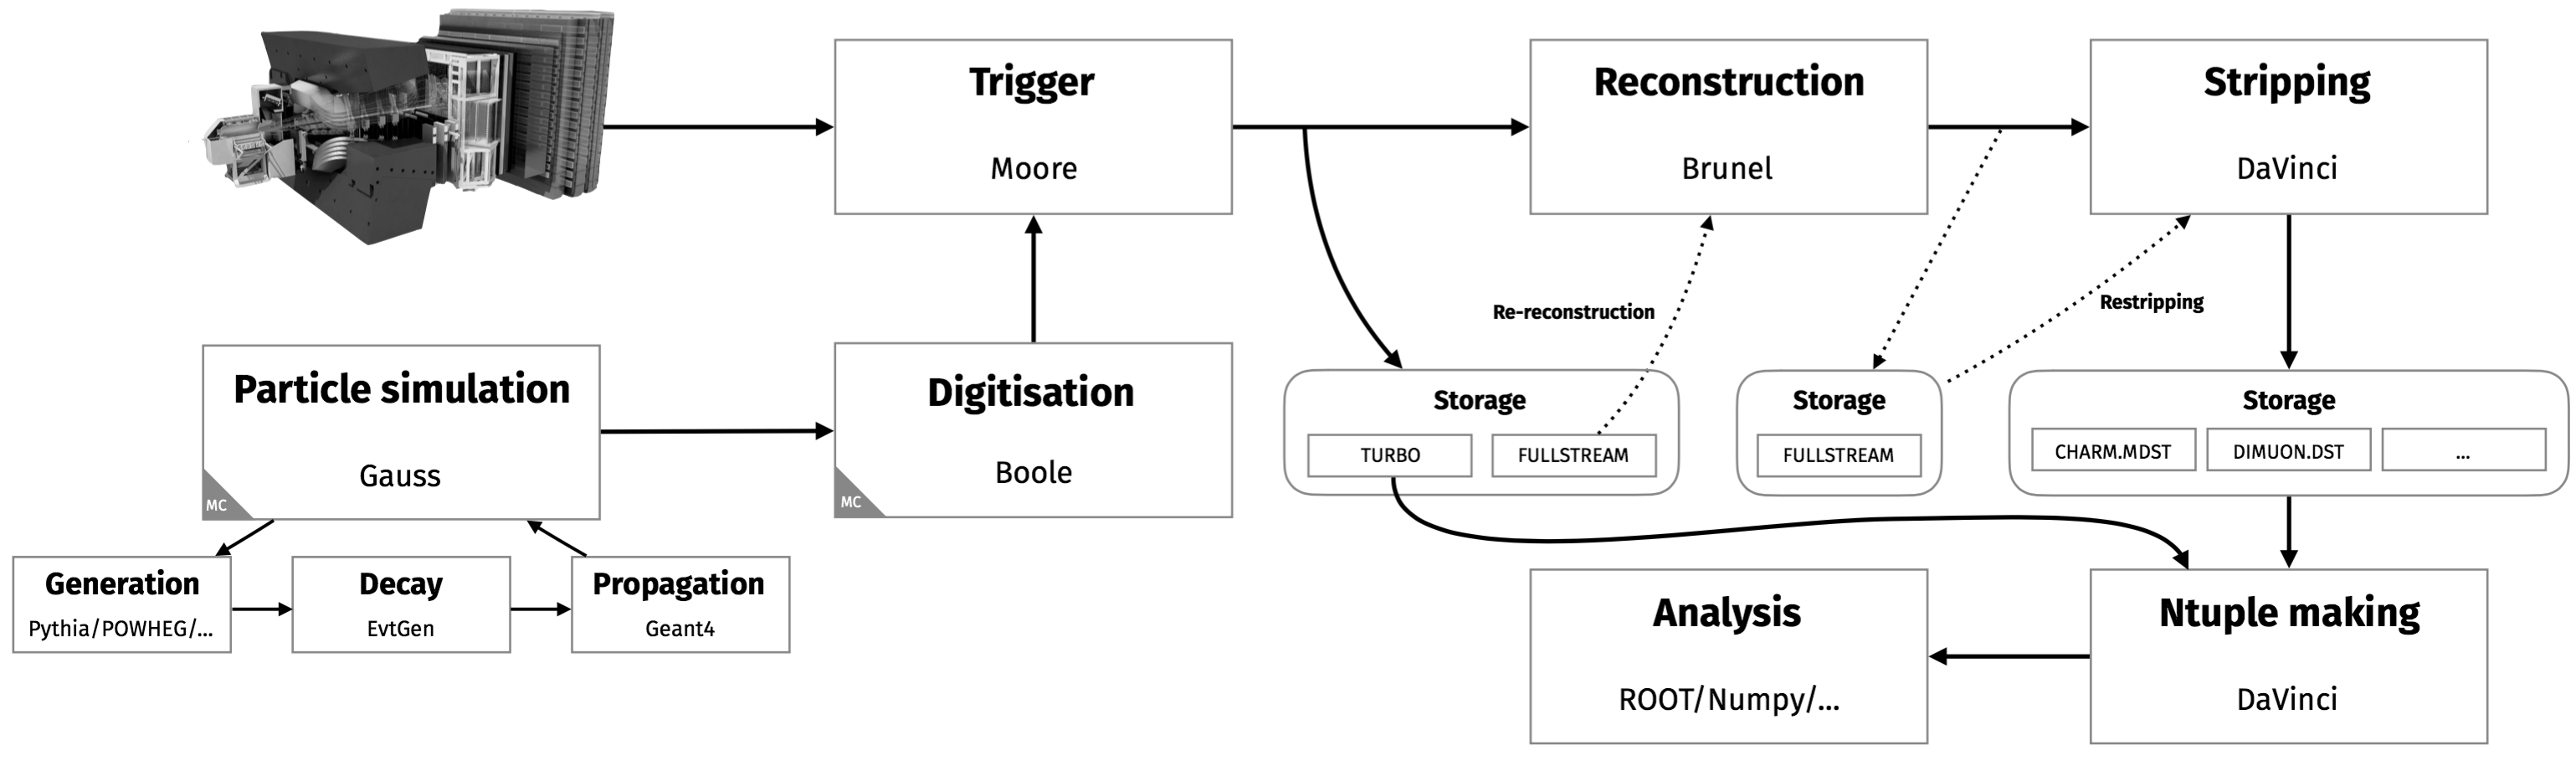
\includegraphics[width=\textwidth]{graphics/02-lhcb/lhcb_run_2_data_flow.png}
	\caption{Diagram of the LHCb Run 2 data flow.}
	\label{fig:2:lhcb_data_flow}
\end{figure}

Considering the complexity of the LHCb detector environment, as seen in Section \ref{sec:2:lhcb_detector}, it should come to no surprise that the data elaboration process is equally multifaceted.
Figure \ref{fig:2:lhcb_data_flow} sketches the data flow approach during LHC Run 2;
while a full discussion of the mechanics is beyond the scope of this thesis, this section aims to provide a basic understanding of the different steps in order to grasp key concepts relevant to the following work.

\subsection{Trigger}
The trigger system \cite{Antunes-Nobrega:630828} provides the first triage of all data recorded by the LHCb detector.
LHC collides proton-proton bunches at a nominal \SI{40}{\mega\hertz} rate, with $\approx 1\%$ resulting in $b\bar{b}$ events of interest for LHCb.
Furthermore, only $\approx 15\%$ of these events will produce a reconstructible $b$ hadron (i.e. with all decay products within the detector acceptance) \cite{HistoryLHCb}, and studies on topics such as CP violation are likely to require decays with small ($\lesssim {10}^{-3}$) branching ratios.
Peak writing speeds for data storage are in the order of a few \si{\kilo\hertz}, making it impossible to save all information even forgoing the high costs this would entail in terms of storage space.
The LHCb trigger system therefore has to skim out the vast majority of uninteresting events with high efficiency, and it needs to be fast about it.

The trigger system employed during LHC Runs 1 and 2 can be broken down into three distinct phases, or \textit{levels}.
First comes Level-0 (L0), which is implemented directly on hardware via custom-made electronics.
Working synchronously with the \SI{40}{\mega\hertz} bunch-crossing rate, the L0 trigger is only able to read three parts of the LHCb detector independently: the VELO pile-up radial modules, used to reject events with multiple primary proton-proton interactions; the calorimeter trigger (L0-Calorimeter), which selects hadron, photon and electron candidates; and the muon trigger (L0-Muon), which obviously selects muons.

The L0-Calorimeter trigger is based on information from all four subdetectors of the calorimeter system (SPD, PS, ECAL and HCAL) and uses it to compute the transverse energy $E_\text{T}$ deposited by incoming particles.
Events with a large number of charged tracks are vetoed based on the number of hits in the SPD to manage the limited computation time allotted for the subsequent trigger levels.
Based on the $E_\text{T}$ measurement, the trigger builds hadron, electron and photon candidates.

Each of the four L0-Muon trigger processors selects the two highest $p_\text{T}$ tracks from its assigned quadrant among candidates crossing all five muon stations.
The single muon trigger sets a threshold on the highest transverse momentum $p_\text{T}$ of the pair, while the dimuon trigger does so on the product of $p_\text{T}$ of both candidates.

After combining all information, the L0 trigger outputs at a maximum rate of \SI{1}{\mega\hertz} fixed by front-end electronics, the majority being used for muon and hadron triggers (electrons and photons only take up $\approx 15\%$ of the L0 output rate).
These data are then sent to the event filter farm (EFF), where the software-based high level trigger (HLT) algorithms, implemented in the Moore application, process them to further reduce the rate for storage:
the first stage (HLT1) gets the rate down to \SI{100}{\kilo\hertz}, while the second (HLT2) outputs at roughly \SI{12.5}{\kilo\hertz}.
Both HLTs are divided in independently operating \textit{trigger lines}, each line consisting of specific selection instructions for a determined class of events.

HLT1 reconstructs Long charged particles with $p_\text{T} > \SI{500}{\mev}$. First it combines VELO hits to form straight line tracks, then it looks for $\geq 3$ TT hits in a region around the straight line extrapolation of the VELO tracks. The small upstream portion of magnetic field allows for momentum determination with a $20\%$ resolution used to reject low-$p_\text{T}$ tracks.
After that, the tracks are extrapolated at the T stations, looking for hits in IT and OT on one side of the straight line VELO-TT extrapolation (depending on the charge estimate).
Finally, all tracks are fit with a Kalman filter with a simplified detector geometry.
At this stage, particle identification is only possible for muons on account of the tight timing constraints.

Owing to the rate reduction performed by HLT1, HLT2 is able to reconstruct the entire event:
reconstruction of charged tracks with $p_\text{T} > \SI{80}{\mev}$ is performed using all tracking sub-detectors (see Section \ref{sec:2:tracking}), along with reconstruction of neutral clusters and implementation of the full particle identification system (Section \ref{sec:2:pid}).

\subsection{From reconstruction to analysis}
The data flow reaches a fork after HLT2.
While the trigger output can be used for data analysis, the hectic timing requirements for said phase mean that only information on the decay of interest for the related HLT2 trigger line is reconstructed, leaving the rest as raw data.

The \textit{full stream} branch rectifies this by performing a slower-paced, offline re-reconstruction of the full decay tree controlled by the Brunel application.
Resulting data are saved in Data Summary Tape (DST) format, with a single event occupying $\approx \SI{150}{kB}$ of space.
These DST files undergo the \textit{stripping} process, carried out by the DaVinci application: this applies dedicated loose selection algorithms (\textit{stripping lines}) and groups events in \textit{streams} (the dimuon stream for $\mu^+\mu^-$ events, for instance) to ease access for data analysis.

The resulting DST files, also referred to as \textit{full} DSTs to distinguish from \textit{reduced} DSTs output by Brunel, can then be processed by the end user through DaVinci to apply their own filter algorithms and extract ROOT nTuples\footnote{ROOT \cite{ANTCHEVA20092499} is an C++ open-source data analysis toolkit developed developed at CERN and popular within the high-energy physics community. A key feature of ROOT is the \texttt{TTree} class (\textit{tree} for simplicity), a C++ object container organized in independent \textit{branches}, or \textit{columns}, and optimized for large data sets. The \texttt{TNtuple} class is a \texttt{TTree} with float variables only.} suitable for physics studies.

During Run 1, the full stream path was the only one available, because HLT2 performed a significantly worse reconstruction than Brunel even on the implemented decays.
This changed in Run 2 with the introduction of the parallel \textit{Turbo stream} \cite{Benson_2015}, i.e. the storage of HLT2 output for direct usage by analysts through DaVinci.
The EFF upgrade conducted during the LS1 increased the HLT2 allotted computation time enough to match HLT2 and Brunel performances;
the key difference between the full and turbo streams is that the latter only saves information on the decay of interest for the related HLT2 trigger line to save storage space, preventing future offline reconstruction of the full decay tree by Brunel.

This change was motivated by the increase in center-of-mass collision energy from \SI{8}{\tev} to \SI{13}{\tev}: the higher $b$- and $c$-production cross-sections mean that more events of interest for LHCb are produced in Run 2 despite the same bunch-crossing frequency.
The Turbo stream allows more saved data to be ready for analysis, while the slower Brunel offline process fulfills the need for reconstruction of decays outside of those implemented in HLT2 trigger lines.

\subsection{Monte Carlo simulations}
\label{sec:2:monte_carlo}
The comparison between experimental results and theory predictions is a critical aspect of physics analysis.
In the case of high-energy physics experiments, the latter rely on the correct simulation of events from collision to detector interaction.

In LHCb, the production of Monte Carlo (MC) data is controlled by the Gauss application, which is in charge of coordinating the several cogs of the simulation machine:
proton-proton collisions are simulated via MC generator software such as \textsc{Pythia} \cite{Pythia2015} and \textsc{POWHEG} \cite{Alioli:2010xd}; the decay of generated particles is described by \textsc{EvtGen} \cite{Ryd:2005zz}, while the \textsc{Geant4} toolkit \cite{AGOSTINELLI2003250} simulates the propagation and interaction with the material using a detailed modelization of the LHCb detector.

As the final step, the simulated hits from the virtual detector in \textsc{Geant4} are digitized using the Boole application, which aims to mimic the real output from the LHCb detector.
This allows simulated data to be processed with the same software as the real one, as described in the earlier paragraphs of this section.

\section{LHCb detector upgrade for Run 3}
\label{sec:2:upgrade}

During LHC Runs 1 and 2, the LHCb experiment has collected $\approx \SI{8}{\per\femto\barn}$ of data.
As much as this has allowed the LHCb Collaboration to achieve impressive results in the heavy-flavour sector and beyond, as touched upon in Section \ref{sec:2:lhcb_detector}, many ongoing analyses are still limited by low statistics.
For this reason, during the LS2, work has been carried out to upgrade the detector in software and hardware with the goal of reaching a \SI{50}{\per\femto\barn} integrated luminosity by the end of Run 3 \cite{Piucci_2017}.

The main feature of this upgrade will be the removal of the L0 hardware trigger in favour of a fully software trigger \cite{CERN-LHCC-2014-016}.
After the performance match between HLT2 and Brunel achieved in Run 2, the high level trigger will see an even more central stage in Run 3, being tasked with full reconstruction of all events of interest in the context of a five-fold increase in operational luminosity (up to \SI{2e33}{\per\centi\meter\squared\per\second}).
To prevent trigger yield saturation with such an increase in luminosity, the LHCb readout rate will be augmented from the current \SI{1}{\mega\hertz} to the LHC bunch crossing rate of \SI{40}{\mega\hertz}.

\begin{figure}[t]
	\centering
	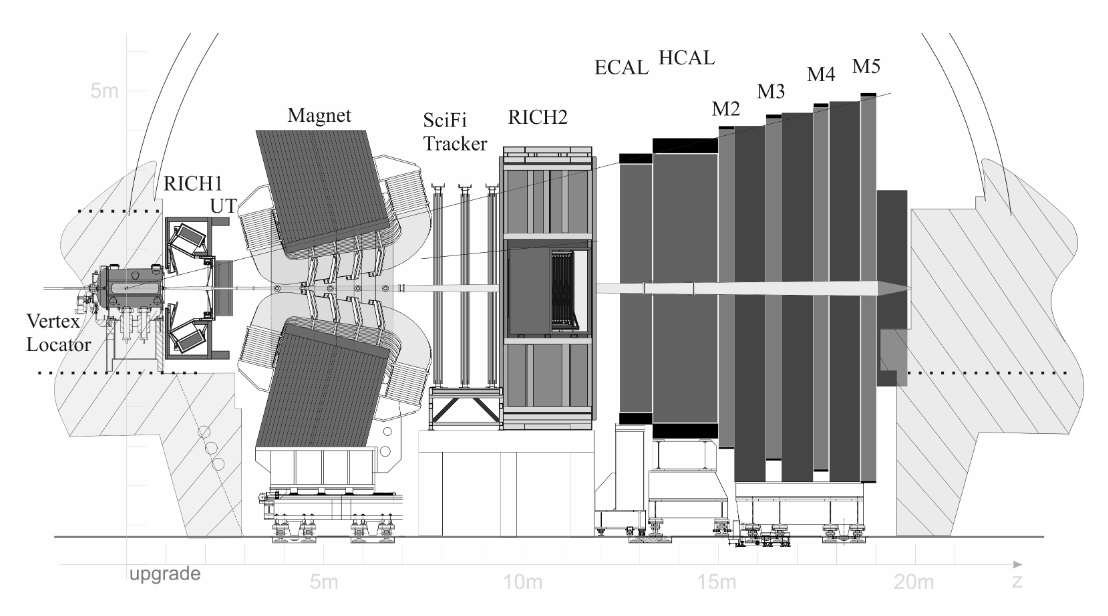
\includegraphics[width=\textwidth]{graphics/02-lhcb/lhcb_diagram_run3.png}
	\caption[LHCb detector side view (Run 3).]{Side view of the upgraded LHCb detector for future usage in LHC Run 3 \cite{Piucci_2017}.}
	\label{fig:2:lhcb_diagram_run3}
\end{figure}

Many parts of the LHCb detector will concurrently be upgraded or partially rebuilt, as seen in Figure \ref{fig:2:lhcb_diagram_run3}, with the most significant changes concerning the tracking system.
The upgraded VELO, also known as VELO Pixel, will replace the silicon microstrip technology with hybrid pixel modules with integrated CO$_2$ cooling, ensuring better radiation hardness, impact parameter resolution and tracking times \cite{Collaboration:1624070}.
Upstream of the magnet, the Upstream Tracker (UT) will take over from the TT, featuring four high granularity silicon microstrip layers with improved coverage of the LHCb angular acceptance. Finally, both inner and outer trackers of the T1--T3 stations will be replaced by the Scintillating Fiber Tracker (SFT or SciFi), based on \SI{2.4}{\meter} plastic scintillating fibers read out by silicon photo-multipliers \cite{Collaboration:1647400}.
This global upgrade is projected to reduce reconstructed fake tracks by as much as $70\%$, drastically shortening trigger timing \cite{Piucci_2017}.

The PID system will also undergo modifications, albeit less substantial ones \cite{Collaboration:1624074}.
Current hybrid photon detectors used in the RICH system cannot be disentangled from the embedded readout electronics operating at \SI{1}{\mega\hertz} and will thus be replaced by commercial multianode photomultipliers;
the optical layout of RICH1 will also be updated to spread gas rings over the entire detector plane, reducing particle occupancy problems\footnote{This is an issue specific to RICH1, being much closer to the interaction point than its downstream counterpart.}.
Whereas the calorimeter system will largely stay the same, muon station M1 will be removed and additional shielding will surround the beam pipe in the M2 region to improve radiation hardness.

\section{Data used for this thesis}
\label{sec:2:used_data}
In the following chapters of this thesis, I will employ data collected during LHCb Run 2, corresponding to an integrated luminosity of \SI{6}{\per\femto\barn}, to conduct studies related to the measurement of the \lz baryon electromagnetic dipole moments pursuing the approach described in Section \ref{sec:lambda}.
The exclusive decay chosen for the analysis is the \lbz channel
\begin{equation*}
	\Lambda_b^0 \rightarrow J/\psi~(\rightarrow \mu^+ \mu^-)~\Lambda^0~(\rightarrow p \pi^-), \tag{\ref{eq:demonstrator_cap1} revisited}
\end{equation*}
exploiting the $\approx 100\%$ longitudinal polarization of the \lz.
This comparatively rare channel ($\text{BR} \approx {10}^{-5}$) is selected at HLT level via the inclusive $J/\psi \rightarrow \mu^+\mu^-$ detached\footnote{The \textit{detached} requirement adds a selection criterium on the muon impact parameters, enforcing their incompatibility with the lowest-$\chi^2$ primary vertex.} trigger line.
The need to measure spin precession in the magnetic field restricts the available \lz to those decaying after the LHCb dipole magnet, implicitly requiring its decay products $p\pi^-$ to be T tracks.

The $\tau \approx \SI{1.5e-12}{\second}$ mean life of the \lbz \cite{PDG} places its decay vertex well inside the VELO detector; in conjunction with the high efficiency reconstruction of muons in LHCb, this justifies a Long track requirement in their case.
The \lbz vertex accuracy afforded by the \jpsi half of the decay chain enables us to impose kinematic constraints on the \lbz half, partially offsetting some of the problems with T tracks I have pointed out in Section \ref{sec:2:tracking}.

Along with Run 2 data, simultated samples of \eqref{eq:demonstrator_cap1} events are used to study the effect of the different steps of signal selection requirements.
These have been generated with \textsc{Pythia} \cite{Pythia2015} using the LHCb-specific configuration implemented in Gauss \cite{Belyaev_2011}, and have been digitized following the procedure detailed in Section \ref{sec:2:monte_carlo}.